\section{Fourierfilterung}
\subsection{Ergebnis}
\subsection{Fourier Schriftzug}
Zuerst soll ein "Fourier" Schriftzug vor einem Gitter modelliert werden, indem das Gitter entfernt wird. Dazu wird eine Tiefpassfilterung benutzt, da die im Vergleich große Schrift hauptsächlich aus niedrigen Frequenzen besteht. 


\begin{figure}[h]
\begin{subfigure}[c]{0.5\textwidth}

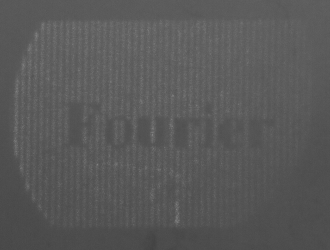
\includegraphics[width=0.9\textwidth]{Fourier.png}
	      \caption{}
          \label{fig:NiceImage1}
          
\end{subfigure}
\begin{subfigure}[c]{0.5\textwidth}
	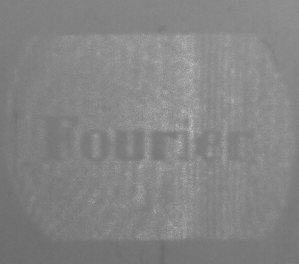
\includegraphics[width=0.9\textwidth]{Fourier_Filter.png}
	      \caption{}
          \label{fig:NiceImage2}
\end{subfigure}
\caption{In \cref{fig:NiceImage1} ist der "Fourier" Schriftzug ohne Filter zusehen; in \cref{fig:NiceImage2} mit einem Tiefpassfilter.}
\label{Fourier}
\end{figure}   

In \cref{Fourier} ist zu sehen, wie sich der Tiefpassfilter auf das Bild auswirkt. Das Gitter ist zum größten Teil nicht mehr als solches zu erkennen.

\subsection{Zähler eines Bruches entfernen}
Daraufhin soll der Zähler eines $\frac{1}{2}$ Bruchs entfernt werden. Wie in \cref{fig:Bruch} zu sehen ist, befindet sich unter dem Zähler ein Gitter, welches sich nicht bei dem Nenner befindet. Es werden also praktisch beide Zahlen entfernt, allerdings ist durch das Gitter immer noch der Umriss der 1 sichtbar. Dieses entfernen geschieht durch eine Hochpassfilterung 

\begin{figure}[h]
	\begin{subfigure}[c]{0.5\textwidth}
		
		\includegraphics[width=0.6\textwidth]{Bruch.png}
		\caption{}
		\label{fig:Bruch}
		
	\end{subfigure}
	\begin{subfigure}[c]{0.5\textwidth}
		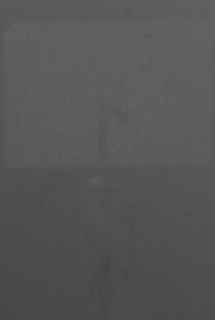
\includegraphics[width=0.58\textwidth]{Filter_Bruch.png}
		\caption{}
		\label{fig:Bruch_filter}
	\end{subfigure}
	\caption{In \cref{fig:Bruch_Filter} ist der "Fourier" Schriftzug ohne Filter zusehen; in \cref{fig:NiceImage2} mit einem Tiefpassfilter.}
	\label{Fourier}
\end{figure}   